\documentclass{article}
\usepackage[paperwidth=14.25in,paperheight=8.35in,margin=0.06in]{geometry}
\usepackage{amsmath}
\usepackage{tikz}
\usetikzlibrary{arrows.meta,positioning,calc}
\pagestyle{empty}
\pgfdeclarelayer{panelbg}
\pgfdeclarelayer{backline}
\pgfsetlayers{panelbg,backline,main}

\begin{document}
\noindent
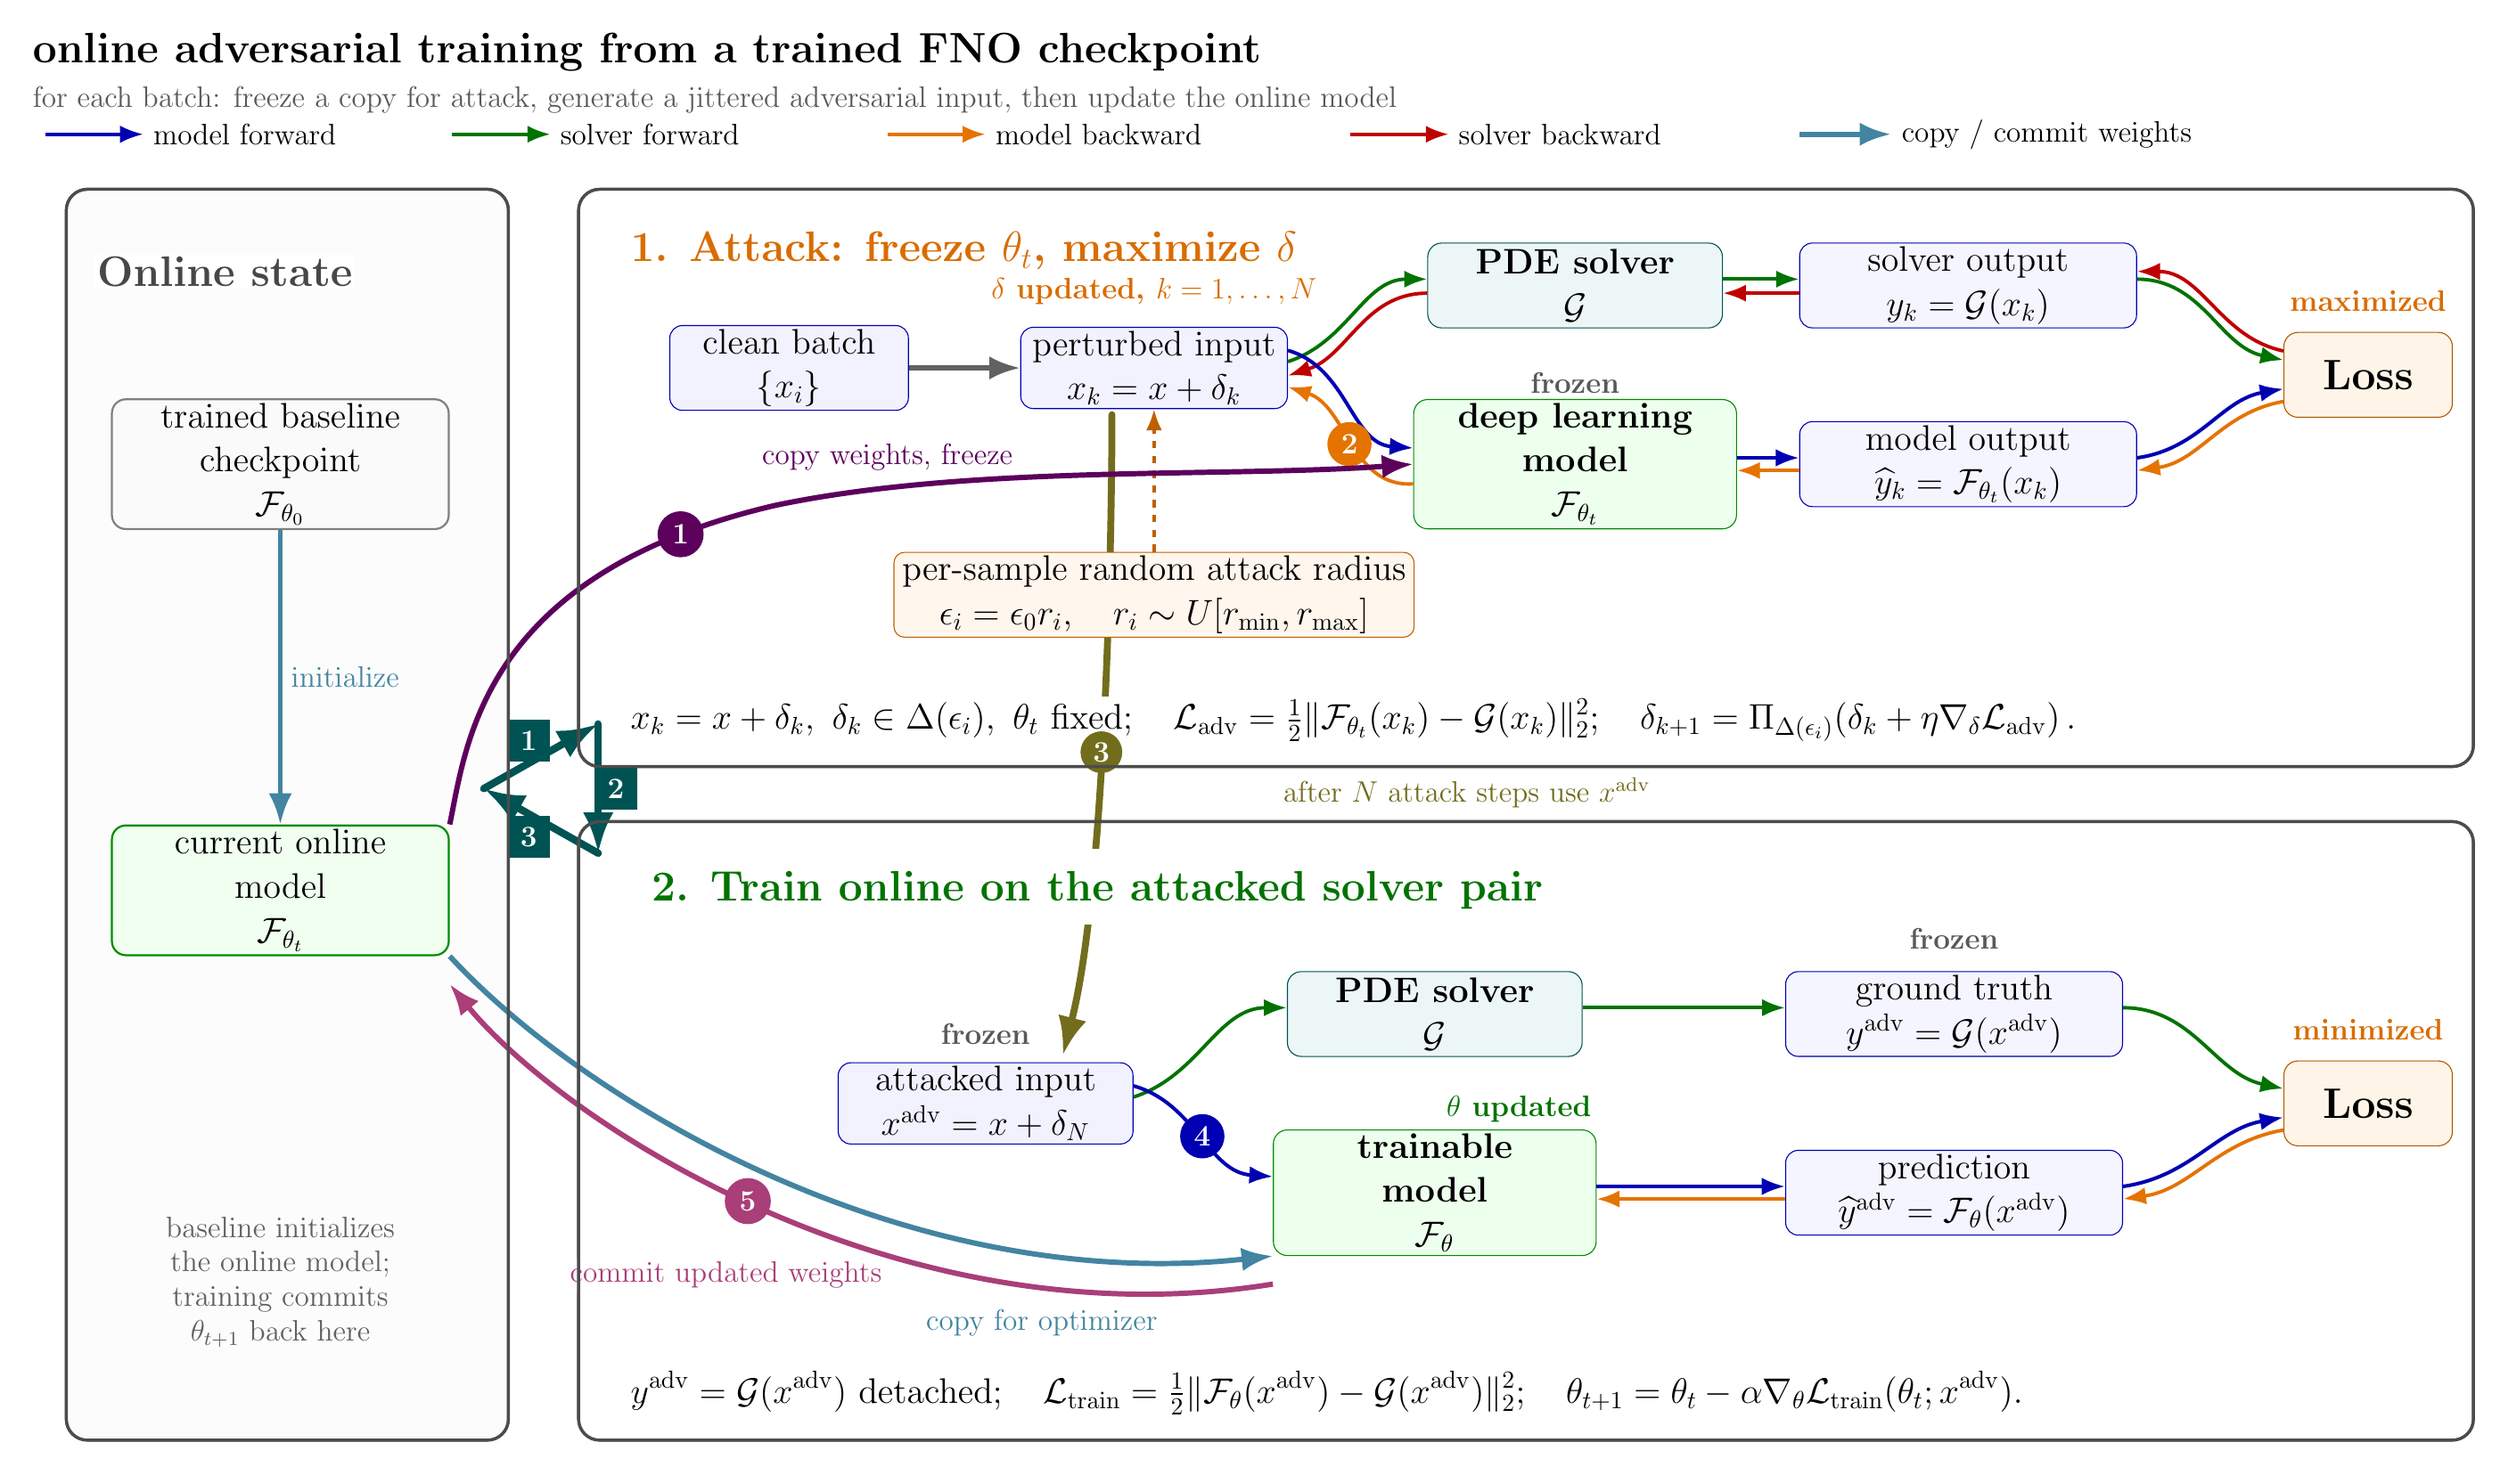
\begin{tikzpicture}[
  x=1mm,y=0.98mm,
  >=Latex,
  font=\sffamily,
  panel/.style={draw=black!65, rounded corners=3mm, line width=1.05pt, fill=white},
  state/.style={draw=black!50, rounded corners=2mm, line width=0.8pt, fill=black!2, minimum width=46mm, minimum height=12.1mm, align=center, font=\Large, inner ysep=1.5pt},
  input/.style={draw=blue!70!black, rounded corners=1.8mm, fill=blue!5, minimum width=37mm, minimum height=11mm, align=center, font=\Large, inner ysep=1.4pt},
  solver/.style={draw=teal!65!black, rounded corners=2mm, fill=teal!7, minimum width=42mm, minimum height=12.1mm, align=center, font=\Large\bfseries, inner ysep=1.4pt},
  model/.style={draw=green!55!black, rounded corners=2mm, fill=green!7, minimum width=46mm, minimum height=13.2mm, align=center, font=\Large\bfseries, inner ysep=1.4pt},
  outbox/.style={draw=blue!70!black, rounded corners=1.8mm, fill=blue!4, minimum width=48mm, minimum height=11mm, align=center, font=\Large, inner ysep=1.4pt},
  loss/.style={draw=orange!70!black, rounded corners=2mm, fill=orange!9, minimum width=24mm, minimum height=12.1mm, align=center, font=\LARGE\bfseries, inner ysep=1.3pt},
  epsbox/.style={draw=orange!75!black, rounded corners=1.5mm, fill=orange!7, minimum width=73mm, minimum height=12.1mm, align=center, font=\Large, inner ysep=1.2pt},
  label/.style={font=\LARGE\bfseries, anchor=west, fill=white, inner sep=1pt},
  formula/.style={font=\Large, anchor=south west, align=left, fill=white, inner sep=1pt},
  note/.style={font=\large, text=black!65, align=left},
  smallnote/.style={font=\large\bfseries, text=black!65, align=center, anchor=south},
  action/.style={font=\large\bfseries, align=center, anchor=south},
  fwd/.style={->, draw=blue!70!black, line width=1.45pt},
  bmodel/.style={->, draw=orange!90!black, line width=1.4pt},
  solverline/.style={->, draw=green!45!black, line width=1.4pt},
  bsolver/.style={->, draw=red!75!black, line width=1.4pt},
  copyarr/.style={->, draw=cyan!60!black, line width=2.15pt},
  copyone/.style={->, draw=violet!72!black, line width=2.15pt},
  copytwo/.style={->, draw=cyan!60!black, line width=2.15pt},
  copythree/.style={->, draw=magenta!65!black, line width=2.15pt},
  macrocycle/.style={->, draw=teal!65!black, line width=3.0pt, line cap=round},
  cyclearr/.style={->, draw=violet!70!black, line width=1.25pt, dashed},
  advbatch/.style={->, draw=olive!75!black, line width=2.8pt, line cap=round},
  thickdata/.style={->, draw=black!62, line width=2.1pt},
  numone/.style={circle, draw=violet!72!black, fill=violet!72!black, text=white, inner sep=1.1pt, minimum size=5.8mm, font=\large\bfseries},
  numorange/.style={circle, draw=orange!90!black, fill=orange!90!black, text=white, inner sep=1.1pt, minimum size=5.8mm, font=\large\bfseries},
  numred/.style={circle, draw=olive!75!black, fill=olive!75!black, text=white, inner sep=1.1pt, minimum size=5.8mm, font=\large\bfseries},
  numblue/.style={circle, draw=blue!70!black, fill=blue!70!black, text=white, inner sep=1.1pt, minimum size=5.8mm, font=\large\bfseries},
  numtwo/.style={circle, draw=cyan!60!black, fill=cyan!60!black, text=white, inner sep=1.1pt, minimum size=5.8mm, font=\large\bfseries},
  numthree/.style={circle, draw=magenta!65!black, fill=magenta!65!black, text=white, inner sep=1.1pt, minimum size=5.8mm, font=\large\bfseries},
  macronum/.style={draw=teal!65!black, fill=teal!65!black, text=white, inner sep=0pt, minimum width=5.9mm, minimum height=5.9mm, font=\large\bfseries}
]

% Title and compact legend
\node[font=\LARGE\bfseries, anchor=west] at (5,204)
  {online adversarial training from a trained FNO checkpoint};
\node[note, anchor=west] at (5,197)
  {for each batch: freeze a copy for attack, generate a jittered adversarial input, then update the online model};

\draw[fwd] (8,192) -- ++(14,0) node[right, black, font=\large] {model forward};
\draw[solverline] (66,192) -- ++(14,0) node[right, black, font=\large] {solver forward};
\draw[bmodel] (128,192) -- ++(14,0) node[right, black, font=\large] {model backward};
\draw[bsolver] (194,192) -- ++(14,0) node[right, black, font=\large] {solver backward};
\draw[copyarr] (258,192) -- ++(13,0) node[right, black, font=\large] {copy / commit weights};

% Left online-state column.
\begin{pgfonlayer}{panelbg}
  \draw[panel, fill=black!1] (11,2) rectangle (74,184);
\end{pgfonlayer}
\node[label, text=black!72] at (15,172) {Online state};
\node[state, minimum width=48mm] (baseline) at (41.5,144)
  {trained baseline\\checkpoint\\$\mathcal F_{\theta_0}$};
\node[state, minimum width=48mm, draw=green!55!black, fill=green!6] (current) at (41.5,82)
  {current online\\model\\$\mathcal F_{\theta_t}$};
\node[font=\large, text=black!62, align=center] at (41.5,25)
  {baseline initializes\\the online model;\\training commits\\$\theta_{t+1}$ back here};
\draw[copyarr] (baseline) -- node[right, font=\large, text=cyan!60!black] {initialize} (current);

% ================= Attack panel =================
\begin{scope}[shift={(84,100)}]
  \begin{pgfonlayer}{panelbg}
    \draw[panel] (0,0) rectangle (270,84);
  \end{pgfonlayer}
  \node[label, text=orange!85!black] at (7,75) {1. Attack: freeze $\theta_t$, maximize $\delta$};

  \node[input, minimum width=34mm] (clean) at (30,58)
    {clean batch\\$\{x_i\}$};
  \node[input, minimum width=38mm] (xin) at (82,58)
    {perturbed input\\$x_k=x+\delta_k$};
  \node[solver] (solver) at (142,70)
    {PDE solver\\$\mathcal G$};
  \node[model] (amodel) at (142,44)
    {deep learning\\model\\$\mathcal F_{\theta_t}$};
  \node[outbox] (ygt) at (198,70)
    {solver output\\$y_k=\mathcal G(x_k)$};
  \node[outbox] (ypred) at (198,44)
    {model output\\$\widehat y_k=\mathcal F_{\theta_t}(x_k)$};
  \node[loss] (aloss) at (255,57) {Loss};

  \node[smallnote, text=orange!85!black] at (82,66.0)
    {$\delta$ updated, $k=1,\ldots,N$};
  \node[smallnote] at (142,53.0) {frozen};
  \node[action, text=orange!85!black] at (255,65.0) {maximized};
  \node[epsbox] (epsnote) at (82,25)
    {per-sample random attack radius\\$\epsilon_i=\epsilon_0 r_i,\quad r_i\sim U[r_{\min},r_{\max}]$};

  \draw[thickdata] (clean) -- (xin);
  \draw[copyarr, dashed, draw=orange!75!black, line width=1.25pt] (epsnote.north) -- (xin.south);

  \draw[solverline] ([yshift=0.9mm]xin.east) to[out=18,in=180] ([yshift=0.9mm]solver.west);
  \draw[solverline] ([yshift=0.9mm]solver.east) -- ([yshift=0.9mm]ygt.west);
  \draw[solverline] ([yshift=0.9mm]ygt.east) to[out=0,in=168] ([yshift=2.1mm]aloss.west);
  \draw[bsolver] ([yshift=3.4mm]aloss.west) to[out=168,in=0] ([yshift=2.0mm]ygt.east);
  \draw[bsolver] ([yshift=-1.1mm]ygt.west) -- ([yshift=-1.1mm]solver.east);
  \draw[bsolver] ([yshift=-1.1mm]solver.west) to[out=180,in=18] ([yshift=-1.1mm]xin.east);

  \draw[fwd] ([yshift=2.5mm]xin.east) to[out=-16,in=176] ([yshift=2.3mm]amodel.west);
  \draw[fwd] ([yshift=0.9mm]amodel.east) -- ([yshift=0.9mm]ypred.west);
  \draw[fwd] ([yshift=0.9mm]ypred.east) to[out=8,in=190] ([yshift=-2.0mm]aloss.west);
  \draw[bmodel] ([yshift=-3.8mm]aloss.west)
    to[out=190,in=8] ([yshift=-0.9mm]ypred.east);
  \draw[bmodel] ([yshift=-0.9mm]ypred.west) -- ([yshift=-0.9mm]amodel.east);
  \draw[bmodel] ([yshift=-2.8mm]amodel.west)
    to[out=184,in=-18]
    node[pos=0.50, numorange] {2}
    ([yshift=-2.7mm]xin.east);

  \node[formula] at (7,3.2)
    {$\displaystyle x_k=x+\delta_k,\ \delta_k\in\Delta(\epsilon_i),\ \theta_t\ {\rm fixed};\quad
      \mathcal L_{\rm adv}=\tfrac12\|\mathcal F_{\theta_t}(x_k)-\mathcal G(x_k)\|_2^2;\quad
      \delta_{k+1}=\Pi_{\Delta(\epsilon_i)}\!\left(\delta_k+\eta\nabla_\delta\mathcal L_{\rm adv}\right).$};
\end{scope}

% ================= Training panel =================
\begin{scope}[shift={(84,2)}]
  \begin{pgfonlayer}{panelbg}
    \draw[panel] (0,0) rectangle (270,90);
  \end{pgfonlayer}
  \fill[white] (8,75) rectangle (156,86);
  \node[label, text=green!45!black] at (10,80) {2. Train online on the attacked solver pair};
  \node[input, minimum width=42mm] (xadv) at (58,49)
    {attacked input\\$x^{\rm adv}=x+\delta_N$};
  \node[solver] (tsolver) at (122,62)
    {PDE solver\\$\mathcal G$};
  \node[model] (tmodel) at (122,36)
    {trainable\\model\\$\mathcal F_\theta$};
  \node[outbox] (tygt) at (196,62)
    {ground truth\\$y^{\rm adv}=\mathcal G(x^{\rm adv})$};
  \node[outbox] (typred) at (196,36)
    {prediction\\$\widehat y^{\rm adv}=\mathcal F_\theta(x^{\rm adv})$};
  \node[loss] (tloss) at (255,49) {Loss};

  \node[smallnote, text=gray!70!black, fill=white, inner sep=1pt] at (58,57.2) {frozen};
  \node[smallnote] at (196,70.2) {frozen};
  \node[smallnote, text=green!45!black] at (134,45.0) {$\theta$ updated};
  \node[action, text=orange!85!black] at (255,57.0) {minimized};

  \draw[solverline] ([yshift=0.9mm]xadv.east) to[out=18,in=180] ([yshift=0.9mm]tsolver.west);
  \draw[solverline] ([yshift=0.9mm]tsolver.east) -- ([yshift=0.9mm]tygt.west);
  \draw[solverline] ([yshift=0.9mm]tygt.east) to[out=0,in=168] ([yshift=2.1mm]tloss.west);
  \draw[fwd] ([yshift=2.5mm]xadv.east)
    to[out=-16,in=176]
    node[pos=0.50, numblue] {4}
    ([yshift=2.3mm]tmodel.west);
  \draw[fwd] ([yshift=0.9mm]tmodel.east) -- ([yshift=0.9mm]typred.west);
  \draw[fwd] ([yshift=0.9mm]typred.east) to[out=8,in=190] ([yshift=-2.0mm]tloss.west);

  \draw[bmodel] ([yshift=-3.8mm]tloss.west)
    to[out=190,in=8] ([yshift=-0.9mm]typred.east);
  \draw[bmodel] ([yshift=-0.9mm]typred.west) -- ([yshift=-0.9mm]tmodel.east);

  \node[formula] at (7,3.2)
    {$\displaystyle y^{\rm adv}=\mathcal G(x^{\rm adv})\ {\rm detached};\quad
      \mathcal L_{\rm train}=\tfrac12\|\mathcal F_\theta(x^{\rm adv})-\mathcal G(x^{\rm adv})\|_2^2;\quad
      \theta_{t+1}=\theta_t-\alpha\nabla_\theta\mathcal L_{\rm train}(\theta_t;x^{\rm adv}).$};
\end{scope}

% Small panel-level cycle: Online state -> Attack -> Train -> Online state.
\draw[macrocycle] (70.5,96.8) -- (86.8,106.2);
\node[macronum] at (76.9,103.8) {1};
\draw[macrocycle] (86.8,106.2) -- (86.8,87.4);
\node[macronum] at (89.3,96.8) {2};
\draw[macrocycle] (86.8,87.4) -- (70.5,96.8);
\node[macronum] at (76.9,89.8) {3};

% Model-copy triangle and attack-to-training handoff.
\draw[copyone] (current.north east)
  .. controls (68,103) and (70,128) ..
  node[pos=0.88, numone] {1}
  (112,138)
  .. controls (140,144) and (176,142) ..
  (amodel.west);
\node[font=\large, text=violet!72!black, fill=white, inner sep=1.5pt]
  at (128,145) {copy weights, freeze};

\draw[copytwo] (current.south east)
  .. controls (84,52) and (130,23) ..
  (tmodel.south west);

\draw[copythree] ([yshift=-4mm]tmodel.south west)
  .. controls (130,16) and (82,48) ..
  node[pos=0.52, numthree] {5}
  ([yshift=-4mm]current.south east);
\node[font=\large, text=cyan!60!black, fill=white, inner sep=1.5pt]
  at (150,19) {copy for optimizer};
\node[font=\large, text=magenta!65!black, fill=white, inner sep=1.5pt]
  at (105,26) {commit updated weights};

\begin{pgfonlayer}{backline}
\draw[advbatch] ([xshift=-6mm,yshift=-0.8mm]xin.south)
  .. controls (160,132) and (159,82) ..
  coordinate[pos=0.54] (advthreeoncurve)
  ([xshift=11mm,yshift=1mm]xadv.north);
\end{pgfonlayer}
\node[numred] at (advthreeoncurve) {3};
\node[font=\large, text=olive!75!black, fill=white, inner sep=1.0pt, anchor=west]
  at (184,96.2) {after $N$ attack steps use $x^{\rm adv}$};

% Redraw the online-state and main panel borders on the foreground so vertical edges stay dark.
\draw[draw=black!70, rounded corners=3mm, line width=1.25pt, line join=round] (11,2) rectangle (74,184);
\draw[draw=black!70, line width=1.25pt, line cap=round] (11,5) -- (11,181);
\draw[draw=black!70, line width=1.25pt, line cap=round] (74,5) -- (74,181);
\draw[draw=black!70, rounded corners=3mm, line width=1.25pt] (84,100) rectangle (354,184);
\draw[draw=black!70, rounded corners=3mm, line width=1.25pt] (84,2) rectangle (354,92);

\end{tikzpicture}
\end{document}
